\documentclass[a4paper, 12pt]{article}%тип документа

%%%Библиотеки
	%\usepackage[warn]{mathtext}	
	\usepackage[T2A]{fontenc} % кодировка
	\usepackage[utf8]{inputenc} % кодировка исходного текста
	\usepackage[english,russian]{babel} % локализация и переносы
	\usepackage{caption}
	\usepackage{listings}
	\usepackage{amsmath,amsfonts,amssymb,amsthm,mathtools}
	\usepackage{wasysym}
	\usepackage{graphicx}%Вставка картинок правильная
	\usepackage{float}%"Плавающие" картинки
	\usepackage{wrapfig}%Обтекание фигур (таблиц, картинок и прочего)
	\usepackage{fancyhdr} %загрузим пакет
	\usepackage{lscape}
	\usepackage{xcolor}
	\usepackage[normalem]{ulem}
	\usepackage{hyperref}

%%%Конец библиотек




%%%Настройка ссылок
	\hypersetup
	{
		colorlinks=true,
		linkcolor=blue,
		filecolor=magenta,
		urlcolor=blue
	}
%%%Конец настройки ссылок


%%%Настройка колонтитулы
	\pagestyle{fancy}
	\fancyhead{}
	\fancyhead[L]{Лабораторная работа}
	\fancyhead[R]{Талашкевич Даниил, группа Б01-009}
	\fancyfoot[C]{\thepage}
%%%конец настройки колонтитулы



							\begin{document}
						%%%%Начало документа%%%%


%%%Начало титульника
\begin{titlepage}

	\newpage
	\begin{center}
		\normalsize Московский физико-технический институт \\(госудраственный 			университет)
	\end{center}

	\vspace{6em}

	\begin{center}
		\Large Лабораторная работа по электричеству\\
	\end{center}

	\vspace{1em}

	\begin{center}
		\large \textbf{Закон Кюри-Вейсса [3.4.2]}
	\end{center}

	\vspace{2em}

	\begin{center}
		\large Талашкевич Даниил Александрович\\
		Группа Б01-009
	\end{center}

	\vspace{\fill}

	\begin{center}
	Долгопрудный \\2021
	\end{center}
	
\end{titlepage}
%%%Конец Титульника



%%%Настройка оглавления и нумерации страниц
	\thispagestyle{empty}
	\newpage
	\tableofcontents
	\newpage
	\setcounter{page}{1}
%%%Настройка оглавления и нумерации страниц


					%%%%%%Начало работы с текстом%%%%%%
					
\textbf{Цель работы} : изучение температурной зависимости магнитной восприимчивости ферромагнетика выше точки Кюри.

\textbf{В работе используются} : катушка самоиндукции с образцом из гадолиния, термостат, частотомер, цифровой вольтметр, $L C$-автогенератор, термопара медь-константан.
                    
\section{Теоретическое введение}


Коэффициент самоиндукции катушки $L$ пропорционален магнитной проницаемости $\mu$ заполняющей его среды (почему?): $L \propto \mu$. Тогда разность самоиндукций катушки с образцом $L$ и без него $L_{0}$ будет пропорциональна восприимчивости образца $\chi$ :
$$
L-L_{0} \propto \mu-1=\chi
$$
При изменении индуктивности образца меняется период колебаний автогенератора:
$$
\tau=2 \pi \sqrt{L C}
$$
где $C$ - ёмкость контура автогенератора. Период колебаний в отсутствие образца определяется самоиндукцией пустой катушки:
$$
\tau_{0}=2 \pi \sqrt{L_{0} C}
$$
Отсюда находим

$$
L-L_{0} \propto \tau^{2}-\tau_{0}^{2}
$$
и, следовательно,
$$
\chi \propto \tau^{2}-\tau_{0}^{2}
$$
Из формул 2 и 3 следует, что закон Кюри-Вейсса справедлив, если выполнено соотношение
$$
\frac{1}{\tau^{2}-\tau_{0}^{2}} \propto T-\Theta_{p}
$$
Измерения проводятся в интервале температур от $14^{\circ} \mathrm{C}$ до $40^{\circ} \mathrm{C}$. С целью экономии времени следует начинать измерения с низких температур.



\section{Экспериментальная установка}

В работе изучается температурная зависимость $\chi(T)$ гадолиния при температурах выше точки Кюри. Выбор материала определяется тем, что его точка Кюри лежит в диапазоне комнатных температур.

\begin{figure}[h!]
    \centering
	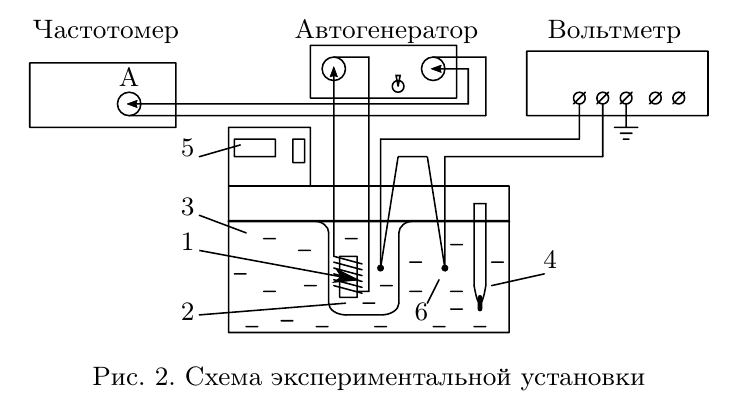
\includegraphics[width = \textwidth]{1.png}
    \caption{Схемы экспериментальных установок}
    \label{scheme}
\end{figure}

Схема установки для проверки закона Кюри-Вейсса показана на рис. 2 Исследуемый ферромагнитный образец (гадолиний) расположен внутри пустотелой катушки самоиндукции, которая служит индуктивностью колебательного контура, входящего в состав $L C$-автогенератора (генератора колебаний с самовозбуждением).

Гадолиний является хорошим проводником электрического тока, а рабочая частота генератора достаточно велика $(\sim 50$ кГц), поэтому для уменьшения вихревых токов образец изготовлен из мелких кусочков размером около 0,5 мм. Катушка 1 с образцом помещена в стеклянный сосуд 2, залитый трансформаторным маслом. Масло предохраняет образец от окисления и способствует ухудшению электрического контакта между отдельными частичками образца. Кроме того, оно улучшает тепловой контакт между образцом и термостатируемой (рабочей) жидкостью 3 в термостате. Ртутный термометр 4 используется для приближенной оценки температуры. Температура образца регулируется с помощью термостата 5 .


\section{Ход работы}

Зная температурный коэффициент термопары (указан на установке), оценим допустимую ЭДС термопары, если допустимая разность температур образца и рабочей жидкости $\Delta T=0,5^{\circ} \mathrm{C}$. Получили допустимую ЭДС термопары $0,02$ мВ.

Исследуем зависимость периода колебаний $LC$ - генератора от температуры образца, отмечая период колебаний $\tau$ по частотомеру, а температуру $T$ -- по показаниям дисплея и цифровому вольтметру ($\Delta U$ с учётом знака). Термопара подключена так, что при знаке "+" на табло вольтметра температура образца выше температуры рабочей жидкости.
Измерения будем проводить в диапазоне от $14^{\circ} \mathrm{C}$ до $40^{\circ} \mathrm{C}$.

Запишем период колебаний $\tau_{0}$ без образца, указанный на установке. $\tau_{0} = 8,252$ мксек.

\section{Обработка результатов}

Рассчитаем температуру $T$ образца с учётом показаний термопары. Таблица полученных результатов

\begin{center}
\begin{table}[!h]
\begin{tabular}{|c|c|c|c|c|c|c|}
\hline Т, $^{\circ} C$ & Т, мксек & $\Delta V$, мВ & $\Delta T$ & T' & $T^2-T_0^2$ & $\frac{1}{T^2-T_0^2}$ \\
\hline 16 & 9,961605 & 0,01 & 0,24 & 16,24 & 31,138070 & 0,032115 \\
\hline 18 & 9,741592 & -0,01 & $-0,24$ & 17,76 & 26,803110 & 0,037309 \\
\hline 20 & 9,456648 & $-0,02$ & $-0,48$ & 19,52 & 21,332687 & 0,046876 \\
\hline 22 & 9,082511 & $-0,02$ & $-0,48$ & 21,52 & 14,396502 & 0,069461 \\
\hline 24 & 8,744112 & $-0,01$ & $-0,24$ & 23,76 & 8,363990 & 0,119560 \\
\hline 26 & 8,605521 & $-0,01$ & $-0,24$ & 25,76 & 5,959487 & 0,167799 \\
\hline 28 & 8,533765 & $-0,02$ & $-0,36$ & 27,64 & 4,729641 & 0,211432 \\
\hline 30 & 8,486562 & $-0,02$ & $-0,36$ & 29,64 & 3,926230 & 0,254697 \\
\hline 32 & 8,461724 & $-0,01$ & $-0,24$ & 31,76 & 3,505269 & 0,285284 \\
\hline 34 & 8,447512 & $-0,01$ & $-0,24$ & 33,76 & 3,264954 & 0,306282 \\
\hline 36 & 8,418071 & $-0,04$ & $-0,96$ & 35,04 & 2,768415 & 0,361217 \\
\hline 38 & 8,407322 & $-0,01$ & $-0,24$ & 37,76 & 2,587559 & 0,386464 \\
\hline 40 & 8,403764 & $-0,11$ & $-2,64$ & 37,36 & 2,527745 & 0,395609 \\
\hline
\end{tabular}
\end{table}
\end{center}

Построим график зависимости $1 /\left(\tau^{2} - \tau_{0}^{2}\right)=f(T)$. Экстраполируя полученную прямую к оси абсцисс , определим парамагнитную точку Кюри $\Theta_{p}$ для гадолиния.

\begin{figure}[h!]
    \centering
	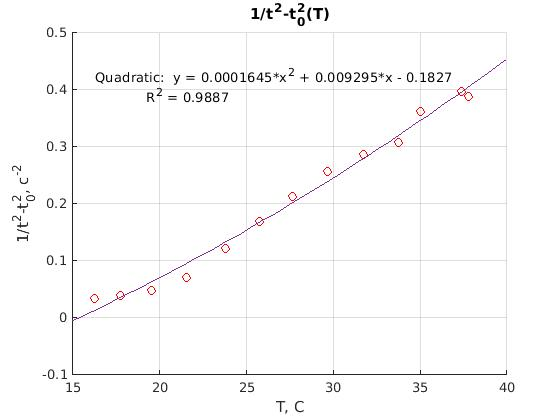
\includegraphics[scale = 0.5]{g1.jpg}
    \caption{квадратичная аппроксимация зависимости $1 /\left(\tau^{2}-\tau_{0}^{2}\right)$ от температуры }
    \label{scheme}
\end{figure}

\begin{figure}[h!]
    \centering
	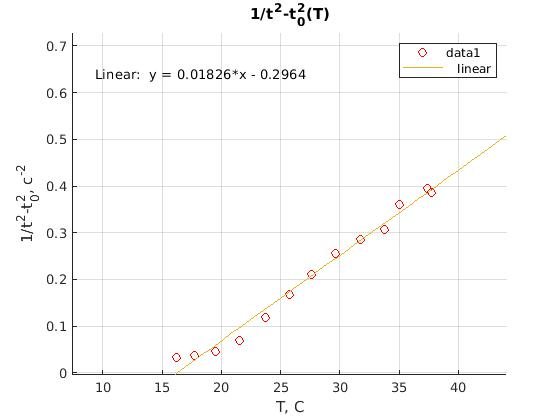
\includegraphics[scale = 0.5]{linAppr.jpg}
    \caption{линейная аппроксимация зависимости $1 /\left(\tau^{2}-\tau_{0}^{2}\right)$ от температуры }
    \label{scheme}
\end{figure}

\[ y = 0,01826x - 0,2964 \Rightarrow [y(x) = 0]\ x = 16,24\ ^{\circ} C \]

В свою очередь табличное значение парамагнитной -- 18,85, ферромагнитной -- 20,2. Данные были получены из лабораторного практикума, а так же на сайте $amtc.ru$ .

\begin{figure}[!h]
    \centering
	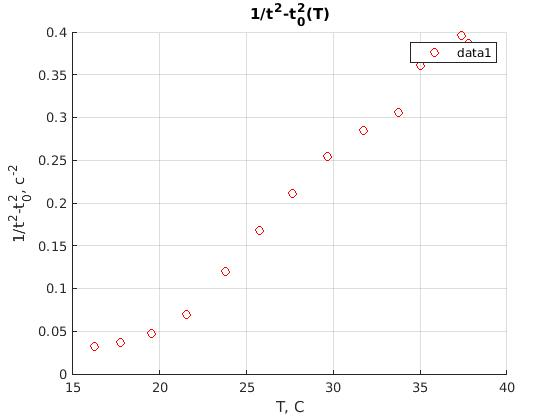
\includegraphics[scale = 0.5]{justPoints.jpg}
    \caption{зависимость $1 /\left(\tau^{2}-\tau_{0}^{2}\right)$ от температуры }
    \label{scheme}
\end{figure}


По участку, отклоняющемуся от линейной зависимости, оценим положение ферромагнитной точки Кюри (как среднее арифметическое между двух соответствующих точек)$\Theta_{\mathrm{K}} \approx \frac{19.52 + 21.52}{2} = 20,52\ ^{\circ}C$.

Погрешность ферромагнитной точки можно для оценки связать погрешность отдельного измерения:

\[  \sigma_T = \sigma_{\text{прибора}} + \sigma_{\text{термопары}} \approx 0,2\ ^{\circ} C\]

\[ \sigma_{\Theta_{\mathrm{K}}} = 2 \cdot \sigma_T = 0,4\ ^{\circ}C\]

Погрешность парамагнитной точки оценим через МНК для линейного участка :

\begin{equation}\label{}
\sigma_{\Theta_p} = \Theta_p \sqrt{\left(\dfrac{\sigma_a}{a}\right)^2 +\left(\dfrac{\sigma_b}{b}\right)^2} = 1,35 ^{\circ} C
\end{equation}

\section{Вывод}

В ходе работы был экспериментально подтвержден закон Кюри-Вейсса для металла гадолиния. Была найдена температура Кюри:

\[ \text{Парамагнитная: } \Theta_{\mathrm{p}} (\text{эксп}) = 16,24 \pm 1,35\ ^{\circ}C\]
\[ \text{Парамагнитная: } \Theta_{\mathrm{p}} (\text{теор}) = 18,85\ ^{\circ}C\]


\[ \text{Ферромагнитная: } \Theta_{\mathrm{K}} (\text{эксп}) = 20,52 \pm 0,4\ ^{\circ}C\]
\[ \text{Ферромагнитная: } \Theta_{\mathrm{K}} (\text{теор}) = 20,2\ ^{\circ}C\]
 
Для ферромагнитной полученное значение лежит от теоретического в доверительном диапазоне, в случае же с парамагнитной полученная величина попадает в порядок, однако лежит в пределах $2\sigma$.

Так же в ходе работы была определена погрешность полученных результатов. Погрешность составила $\varepsilon_{\Theta_{\mathrm{p}}} \approx 8,3 \%$; $\varepsilon_{\Theta_{\mathrm{K}}} \approx 1,9\%$.

Основной вклад в погрешность внесла неточность данных, полученных при температурах, близких к температуре Кюри. Неточность связана с проблемами, возникшими при использовании оборудования для проведения эксперимента.

 
\section{Литература}

\begin{enumerate}

\item \textbf{Лабораторный практикум по общей физике:} Учебное пособие. В трех томах. Т. 2. Электричество и магнетизм /Гладун А.Д., Александров Д.А., Берулёва Н.С. и др.; Под ред. А.Д. Гладуна - М.: МФТИ, 2007. - 280 с.

\item \text{http://www.amtc.ru/production/metall/Gadoliniy}

\end{enumerate}		
		


\end{document}